\section{Ergebnisse}
\textcolor{red}{• Darstellung der Ergebnisse:
• Tabellen
• Grafiken
• Text
• für Datenanalyse und Simulation}

hier tabellen und graphs
\subsection{Modellwahl}
%Tabelle mit BIC der Modelle, CV Ergebnisse, ggf. Koeffizienten
Es wurde Modell \texttt{lm1} als bestes Modell mit einem BIC von 7,5 ermittelt:\\
\\
$ln(soil.res)=\beta_0+\beta_1\cdot{temp.15}^2+\beta_2\cdot{litter.d}^2+\epsilon$\\
\\
Keine der Interaktionen haben den BIC oder die k-fache Kreuzvalidierung verbessert und werden deswegen
weggelassen. Auch die linearen Terme  \texttt{temp.15} und \texttt{litter.d} haben das Modell verschlechtert
und wurden deswegen und aus Parsimonie Gründen weggelassen.

Abbildung \ref{fig:Residuen} zeigt die Residuen für das Modell. Auf der x-Achse sind die vorhergesagten Werte und auf der y-Achse die Residuen.
\begin{figure}[h]
  \centering
  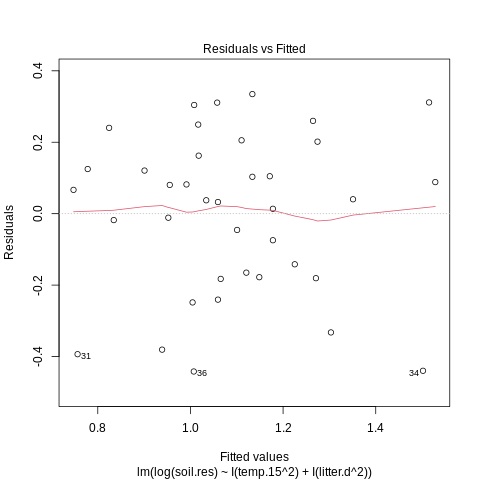
\includegraphics[scale=0.5]{pictures/residuals_lm1.png}
  \caption{Residuenplot des finalen Modells}
  \label{fig:Residuen}
\end{figure}

\subsection{Simulation}

Die Simulationsstudie zeigt, dass ...
